%!TEX root = paper.tex


\begin{table*}\centering
\begin{tabular}{|r|p{2.4in}|p{4in}|}
\hline
& {\bf Spec} & {\bf Meaning} \\
\hline
\hline
1&\small\verb|mpileaks|                         & \small {\tt mpileaks} package, no constraints. \\\hline
2&\small\verb|mpileaks@1.1.2|                   & \small {\tt mpileaks} package, version 1.1.2. \\\hline
3&\small\verb|mpileaks@1.1.2 %gcc|              & \small {\tt mpileaks} package, version 1.1.2, built with {\tt gcc} at the default version. \\\hline
4&\small\verb|mpileaks@1.1.2 %intel@14.1 +debug| & \small {\tt mpileaks} package, version 1.1.2, built with Intel compiler version 14.1, \newline with the ``debug'' build option. \\\hline
5&\small\verb|mpileaks@1.1.2 =bgq|              & \small {\tt mpileaks} package, version 1.1.2, built for the Blue Gene/Q platform (BG/Q). \\\hline
6&\small\verb|mpileaks@1.1.2 ^mvapich2@1.9|     & \small {\tt mpileaks} package version 1.1.2, using {\tt mvapich2}  version 1.9 for MPI. \\\hline
7&\small\verb|mpileaks @1.2:1.4 %gcc@4.7.5 -debug =bgq| \newline
      \verb|  ^callpath @1.1 %gcc@4.7.2| \newline
      \verb|  ^openmpi @1.4.7|                & \small%
      {\tt mpileaks} at any version between 1.2 and 1.4 (inclusive), built with gcc 4.7.5, 
      without the debug option, for BG/Q, linked with {\tt callpath} version 1.1
      and building {\tt callpath} with {\tt gcc} version 4.7.2, linked with {\tt openmpi} version 1.4.7.    \\
\hline
\end{tabular}
\caption{
	Example Spack build specs and their meanings.
	\label{tab:specs}
}
\end{table*}


\begin{figure}
	\subfigure[{\tt mpileaks}]{
		\centering
		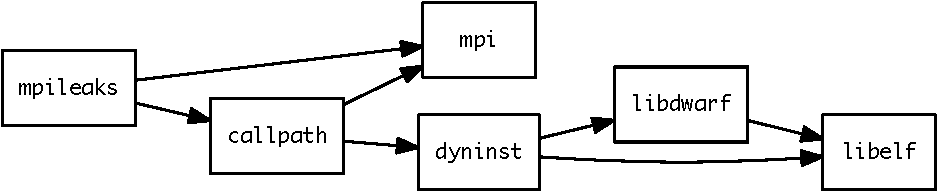
\includegraphics[width=\columnwidth]{specs/mpileaks.pdf}
		\label{fig:specs-mpileaks}
	}
	\subfigure[{\tt mpileaks \^{}callpath\@1.0+debug \^{}libelf\@0.8.11}]{
		\centering
		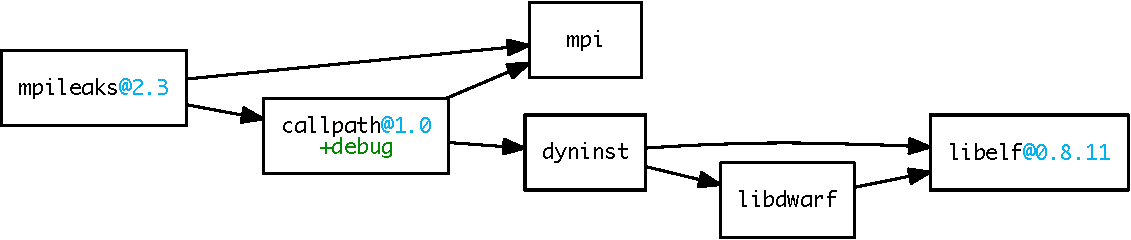
\includegraphics[width=\columnwidth]{specs/mpileaks-abstract.pdf}
		\label{fig:specs-mpileaks-abstract}
	}
	\subfigure[Concrete version of (b)]{
		\centering
		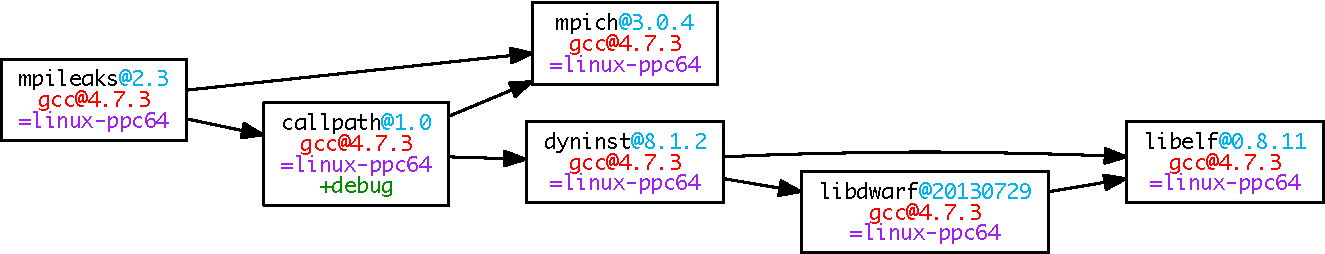
\includegraphics[width=\columnwidth]{specs/mpileaks-concrete.pdf}
		\label{fig:specs-mpileaks-concrete}
	}
	\caption{
		Specs for the {\tt mpileaks} package.
		\label{fig:specs}
	}
\end{figure}


\subsection{Spack Specs}\label{sec:specs}

The package shown in Figure~\ref{fig:mpileaks} seems simple, but even this short script
allows Spack to build many versions of the {\tt mpileaks} package.  This is because builds
in Spack are parameterized.  In traditional port systems, code is structured to build a single
version of a package, but in Spack, each package file is a {\it template} that can build 
in many different ways.  Spack's representation of a configuration is a build specification, 
or {\tt spec}.

\subsubsection{Spec structure}
To understand how specs works, consider the package structure.  The  {\tt Mpileaks} package
is a class, and its metadata ({\tt version}, {\tt depends\_on}, etc.) statically describe
its relationships with other packages.  In this case, there are two direct dependencies: 
the {\tt callpath} library and {\tt mpi}.  Spack recursively inspects the class definitions
for each of these packages to construct a graph of their relationships.  
To avoid issues with incompatible ABIs, and to guarantee a consistent build, the DAG is constructed
so that there is only ever one version of any particular package.

For {\tt mpileaks}, 
the initial graph is shown in Figure~\ref{fig:specs-mpileaks}.  This graph is the in-memory
representation of a spec.

Each package, or node, in the spec has a number of configuration parameters that control
how the package will be built.  These are the version, compiler to build with, compiler version, 
named build options (or {\it variants} like +debug or -debug), and the architecture to
build for.  When Spack runs to install {\tt mpileaks}, it constructs a package object for each node
in the spec DAG, and it traverses the DAG in a bottom-up fashion.  At each node, it
invokes the package's {\tt install()} method, passing in a sub-DAG rooted at the
package to be installed.  This is the {\tt spec} parameter in Figure~\ref{fig:mpileaks}.
Package maintainers are responsible for examining the spec's configuration and adjusting the 
build if necessary.

\subsubsection{Spec syntax}
A spec DAG has many degrees of freedom, and it is not reasonable to expect users to
understand all of them.  In our experience at LLNL, users typically have a small number of 
build constraints that they care about, and the others only confuse them.  This is part of why
the HPC software ecosystem is so difficult to manage: there are simply too many parameters.
However, the small set of important build constraints can be very specific, so we need the
ability to specify all aspects of the configuration space if necessary.  For this reason, 
we introduce a telescoping syntax for package specs that allows users of Spack to
specify {\it only those constraints they care about}, but to be {\it specific when necessary}.
This is the true power of our syntax---specs are concise enough to use on the command line,
and users can request installs or query existing installs by their structure.

Table~\ref{tab:specs} shows examples of specs, ranging from very simple to very complex.
Next to each is a description of the spec in plain language.  In the most basic case,
shown on line 1 in the table, a user can simply name the package they want to use, and have it
built and installed a default configuration.  On the command line this would take the form:
\newline\newline
{\tt spack install mpileaks}
\newline

If the user wants more specificity, {\tt mpileaks} can be augmented with additional
qualifiers.  Spack install will handle selecting a build configuration that satisfies
the user's request.  We describe additional qualifiers below.

{\bf Versions.}
Versions are specified by supplying {\tt @<version>} after the package name (line 2). 
Versions can be precise (e.g. {\tt @4.5.1}) or 
they can be ambiguous (e.g., @4) or a colon-separated, inclusive range (e.g., @4.4:4.5.1),
and Spack will pick an available compiler from the specified range.
The package in Figure~\ref{fig:mpileaks} lists two ``safe'' versions with checksums, but
in our experience users frequently want bleeding-edge versions.  Package managers
frequently lag behind the latest releases. 
Spack has a capability to extrapolate URLs from versions,
using the package's {\tt url} attribute as a model\footnote{This works
for packages with consistently named URLs}.  The user can request a specific
version on the command line, even if it is unknown to Spack,
and Spack will attempt to install it.  Spack also uses the same
model to scrape webpages and find new versions as they become available.

{\bf Compilers.}
To specify the compiler (line 3), the user
simply adds {\tt \%} followed by its name, and if a version {\it of the compiler} 
is desired, the same {\tt @} syntax can be used.  Here, {\tt gcc} refers to the full
gcc compiler suite: C, C++, Fortran 77, and Fortran 90 compilers.  Spack can auto-detect
compiler toolchains if they are in the user's PATH or they can be registered manually
through a configuration file.

{\bf Variants.}
To handle build-time options like debug flags and optional components, spack
allows named flags, or {\it variants} to be associated with packages.  
In the example (line 4), {\tt mpileaks} can be built with a {\tt debug} option by
adding {\tt +debug}.  The option can be similarly disabled with {\tt -debug}.  
This allows package authors to provide package-specific build options without 
having to extend Spack.  We use names for these to simplify the spec
syntax, and to prevent Spack's configuration space from becoming too fine-grained.
It would be violate our goal of conciseness, for example, to include detailed 
compiler flags in the spec syntax, but known sets of flags can be exported using
named variants.

{\bf Cross-compileation.}
To support cross-compilation, Spack includes the platform in the package spec (line 5).
Platforms begin with {\tt =} and take names like {\tt linux-ppc64} or {\tt bgq}.  They are
specified per-package; this allows front-end tools to depend on their back-end measurement
libraries with a {\it different} architecture on cross-compiled machines.

{\bf Dependencies.}
Lines 6 and 7 in the table show the key feature that enables Spack's flexibility.
The user can specify all of the above information not only for the package being
installed, but also for its {\it dependencies}.  To do this, the user needs only supply 
\verb|^| and the dependency's name.  If we need to build a new version with a specific
version of {\tt mvapich2}, we can simply add, e.g., \verb|^mvapich2@1.9|
to the spec, and it will build with that MPI version instead of the default.
This can also be done for multiple libraries in the same spec (line 7).  
As mentioned, Spack guarantees that there is only one version of any package in 
the spec DAG.  So, within the same DAG, each dependency can be uniquely identified by 
only its package name.  This frees the user from having to worry about DAG connectivity;
the user only needs to know that a package depends, somehow, indirectly on {\tt mvapich}
to add this constrain
uniquely identifies a dependency, and dependency constraints can be specified in any
order.  


\subsubsection{Constraining dependencies}


\subsubsection{Build specialization}


\subsubsection{Version extrapolation}


\subsubsection{Querying installed packages}




